\chapter{Diskussion af resultater}

%Her udpeges og diskuteres relevante dele af de opnåede resultater og deres betydning. Der skal også gives en samlet vurdering af de opnåede resultater med relation til projektets problemformulering. Der kan ligeledes være en opsummerende beskrivelse af resultater som I er særligt stolte af.

\section*{Indledning}
Dette afsnit vil diskutere og kommentere relevante resultater og problemstillinger i forbindelse med udvikling af detekteringssystemet.  

\section{Detekteringsalgoritme}
Detekteringsystemet er udviklet til at kunne detektere en frakturering ved en 22 mm Atlas$^\circledR$ Gold ballon og en POM-stent, som simulerer en Mitroflow 21 mm. Det ønskes, at detekteringssystemet kan benyttes til andre ballon- og ringstørrelser, da dette vil give  større grundlag for verificering af systemet og mulighed for klinisk anvendelse.  

I forskningsregi bruger man altid en ballonstørrelse, som er 1 mm større end ringen \cite{baggrund10}. Dog sker det klinisk, at valget af ballonstørrelse vurderes individuelt, og bestemmes ud fra den anatomiske struktur af aortaroden, og især placeringen af koronararterierne. Ballonstørrelsen bliver derfor ikke altid valgt på baggrund af klapstørrelsen og forholdet herimellem kan derfor variere.

Til sidst i udviklingen af detekteringssystemet blev det testet, hvorvidt detekteringssystemet kunne detektere en POM-stent frakturering med en 20 mm Atlas$^\circledR$ Gold ballon. Her var det tydeligt, at forholdet mellem POM stenten og ballonen har stor indflydelse på udseendet af det transiente trykfald. Ved dette scenarie var der meget stor variation på udseendet af det transiente trykfald og detekteringssystemet kunne derfor ikke konsekvent detektere en fraktur. På Figur \ref{20ikke} ses det, at amplituden ikke oversteg threshold på 4 og der bliver derfor ikke detekteret en frakturering. På Figur \ref{20detekt} ses det, at amplituden er over threshold på 4 og der bliver derfor detekteret en frakturering. Det ses altså, at der er stor variation og usikkerhed om, hvorvidt der bliver detekteret en frakturering.

\begin{figure}[H]
	\centering
	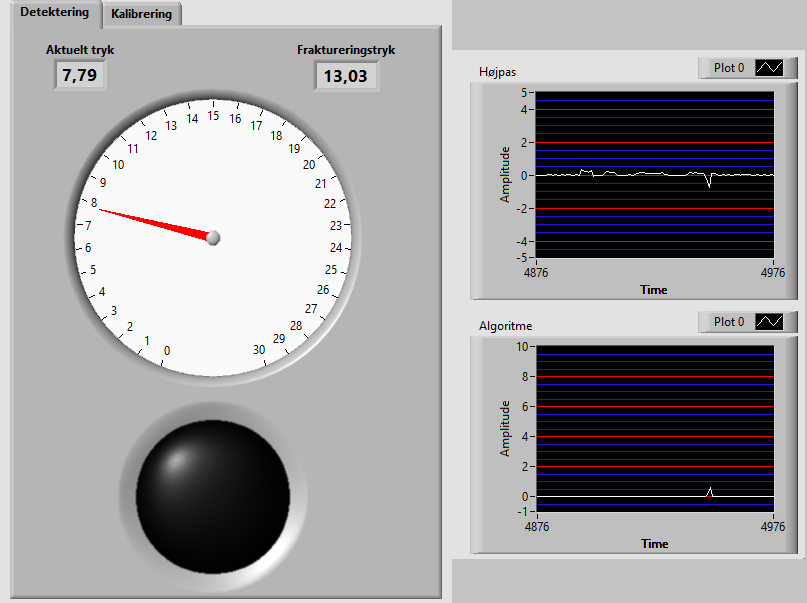
\includegraphics[width=0.6\textwidth]{Figure/20ikke}
	\caption{Frakturering med 20 mm Atlas$^\circledR$ Gold ballon hvor fraktur ikke detekteres}
    \label{20ikke}
\end{figure}

\begin{figure}[H]
	\centering
	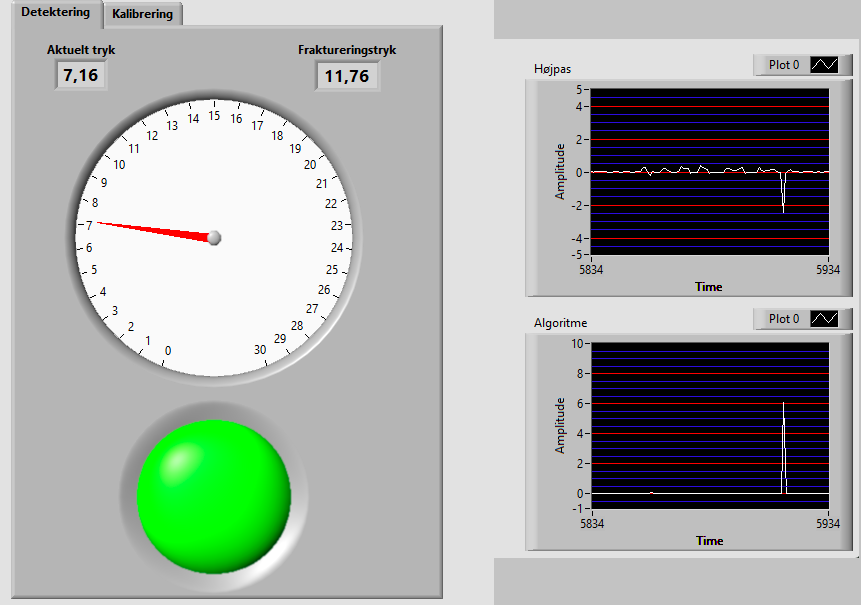
\includegraphics[width=0.6\textwidth]{Figure/20detekt}
	\caption{Frakturering med 20 mm Atlas$^\circledR$ Gold ballon hvor fraktur detekteres}
    \label{20detekt}
\end{figure}

På baggrund af denne observation samt på baggrund af accepttestens Use Case 2, se Kapitel \ref{resultat}, kan det konkluderes, at det udviklede detekteringssystem ikke fungerer optimalt ved andre ballon- og klapstørrelses kombinationer end den, hvorfra detekteringssystemet er blevet udviklet efter. I videre udvikling ønskes det at udvikle en stærkere algoritme, hvormed alle klap og ballon kombinationer detekteres. 


Optimalt burde detekteringsalgoritmen have flere markører, som indikerer, at en frakturering har fundet sted. I Forstudie 1.4 se dokumentation afsnit 9.5 og Bilag 8, blev det undersøgt, hvorledes det transiente trykfald ser ud i de fire scenarier: fri luft, grisseaorta, 3D printet model og hurtig inflatering. Her viste det sig, at det transiente trykfald er meget ensartet i de fire scenarier. Dermed kunne krydskorrelation være en mulig metode til at gøre detekteringsalgoritmen endnu stærkere. 

En alternativ løsning til udvikling af én algoritme kunne være, at der udvikles specifikke algoritmer til den aktuelle procedurer. Hermed skal operatøren indtaste oplysninger om den valgte ballon-type og størrelse samt hvilken hjerteklap, der skal fraktureres. På baggrund af de indtastede oplysninger udvælger detekteringssystemet den algoritme, som vil fungere mest optimal til den aktuelle procedure.  

\section{Tryktransducer}
Til udviklingen af prototypen af detekteringssystemet blev tryktransduceren, Grundfoss pressure transmitter AKS 32 anvendt. Denne tryktransducer blev valgt, da den kan måle de nødvendige fraktureringstryk. Denne tryktransducer kan dog ikke benyttes i klinisk miljø, da den ikke er et godkendt medicinsk udstyr, derfor kan den kun anvendelig til prototypen. Derudover sammenholdes tilslutningen mellem trevejshanen og tryktransduceren udelukkende ved friktion. Denne sammenkobling er ikke en optimal og holdbar løsning, da der ved et tryk over 15 atm lækkes vand fra sammenkobling. Det har i dette projekt ikke været nødvendigt at måle tryk højere end 15 atm og den anvendte tryktransducer har derfor fungeret optimalt til udviklingen af prototypen.   

Som beskrevet tidligere var ikke muligt at bruge den allerede klinisk anvendte tryktransducer. Det vil derfor være relevant at udvikle en tryktransducer, som kan anvendes klinisk, kan måle de nødvendige fraktureringstryk samt kan sammenkobles korrekt til trevejshanen. Formålet med dette projektet har været at udvikle en prototype og den anvendte tryktransducer har derfor fungeret optimalt til dette projekt. 

\section{Lyd notifikation}
Under udviklingen af detekteringssystemet var det essentielt at involvere operatøren og derved medtage hans erfaringer og ønsker til detekteringssystemet. Der blev afholdt usability interview med Jens Erik Nielsen-Kudsk, hvor han blandt andet nævnte, at fraktureringen nogle gange understøttes af en auditiv ”klik”-lyd, som kan høres af operatøren. Det blev derfor valgt at indikere fraktureringen med en klik-lyd, der simulerer det ”klik”, som operatøren intuitivt lytter efter. Endvidere blev det valgt at bruge en lyd, som differentierer sig fra andre lyde på operationsstuen og dermed vil være specifik for netop denne procedurer. 

Lyden blev optaget ved en POM-stent fraktur og er implementeret i detekteringssystemet, så den afspilles, når en frakturering bliver detekteret. Da der i forevejen forekommer mange lyde på operationsstue er det væsentligt, at lyden er hørbar og ikke forveksles med andre lyde. Endvidere er det væsentligt, at lyden ikke bliver et forstyrrende element, men at den opfylder dens egentlige funktion, nemlig at støtte og bekræfte operatøren i, at fraktureringen har fundet sted. Det ville derfor være aktuelt, at udføre et opfølgende usability studie, hvor detekteringssystemet testes i det miljø og brugsscenarie, som det skal implementeres i. 



